\documentclass[10pt,pdf,hyperref={unicode}]{beamer}
\usepackage[utf8]{inputenc}
\usepackage[russian]{babel}
\usepackage{graphicx}
\usetheme{Madrid}

\usenavigationsymbolstemplate{}
\setbeamertemplate{footline}[frame number]

\begin{document}

\title[Детектор объектов]{Детектор объектов}
\subtitle{НИР, весна 2016}
\author{Артем Лобанов \\ Даниил Смирнов \\ Иван Веселов \\ Илья Шевченко \\~\\
        Руководители: Антон Крыщенко, Богдан Бугаев}
\date{31 мая 2016 г.}
\institute{Академический университет}

\begin{frame}
    \titlepage
\end{frame}

\begin{frame}\frametitle{Первый слайд}
    \begin{itemize}
        \item Пункт 1
        \item Пункт 2
        \pause
        \item Выскакивающий пункт
    \end{itemize}
\end{frame}

\begin{frame}\frametitle{Задачи}
    \begin{itemize}
        \item Обеспечить загрузку входных данных
        \item Визуализировать результаты поиска объекта
        \item Склеить написанный код в единый проект
    \end{itemize}
\end{frame}

\begin{frame}\frametitle{Процесс разработки}
    Написаны:
    \begin{itemize}
        \item модуль для загрузки ключевых кадров
        \item интерфейс командной строки для работы с ними
        \item рендер объекта при помощи OpenGL
        \item пользовательский интерфейс для удобства работы
    \end{itemize}
\end{frame}

\begin{frame}\frametitle{Загрузка ключевых кадров}
    \begin{itemize}
        \item Сканирует директорию и ищет в ней объект и ключевые кадры в 
            заданном формате
        \item Считывает их
        \item Выдает класс, содержащий информацию о ключевом кадре --- KeyFrame
    \end{itemize}
    Структура KeyFrame
    \begin{itemize}
        \item Положение и поворот камеры
        \item Внутренние параметры камеры
        \item Положение и поворот объекта
    \end{itemize}
\end{frame}

\begin{frame}\frametitle{GUI. Структура}
    \begin{itemize}
        \item Панель инструментов с кнопками для запуска алгоритмов поиска 
            объекта
        \item Виджет с вкладками, содержащими ключевые кадры
    \end{itemize}
    Структура вкладки:
    \begin{itemize}
        \item Картинка
        \item Модель, отрисованная поверх нее в виде сетки
    \end{itemize}
\end{frame}

\begin{frame}\frametitle{Технологии}
    \begin{itemize}
        \item PySide (Qt) - GUI
        \item OpenGL      - Отрисовка модели объекта на ключевом кадре
    \end{itemize}
\end{frame}

\begin{frame}\frametitle{GUI}
    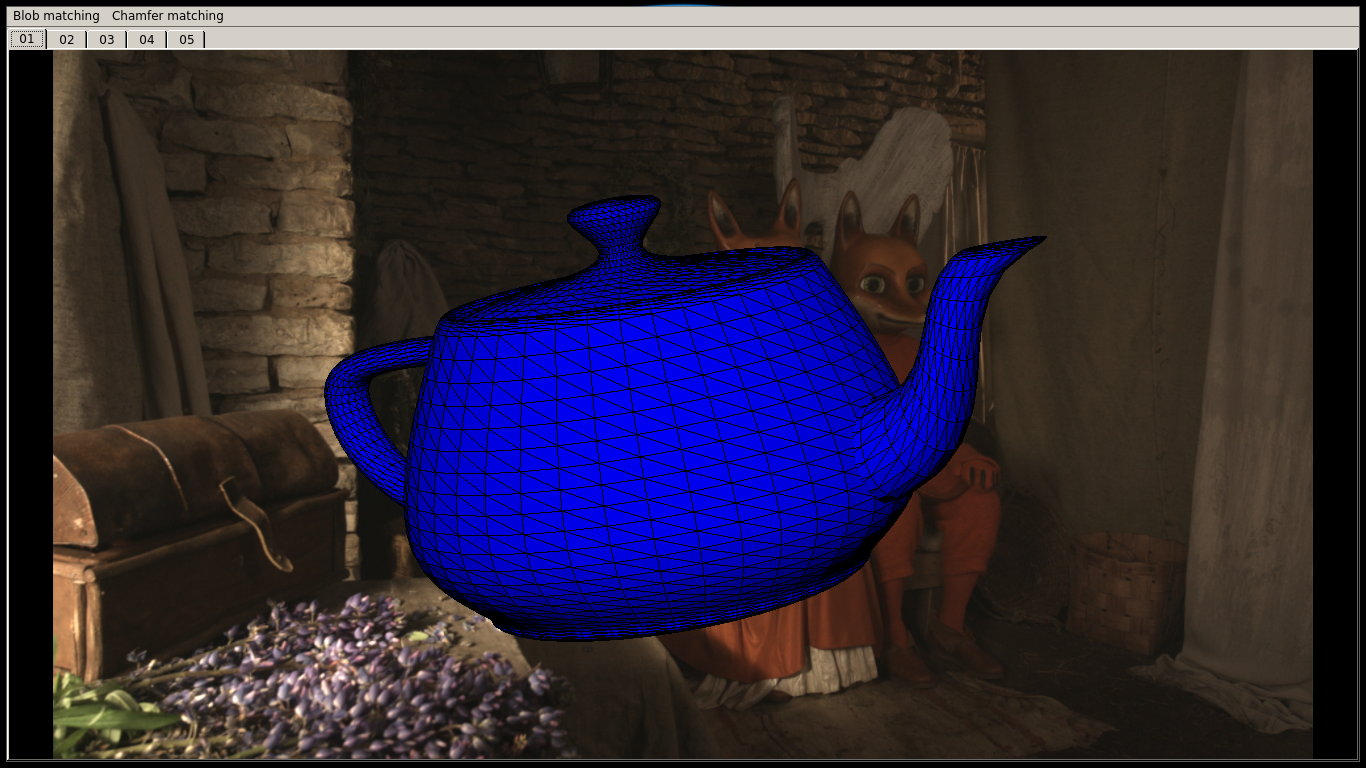
\includegraphics[height=6cm]{gui_samples/sample_01.png}
\end{frame}

\begin{frame}\frametitle{GUI}
    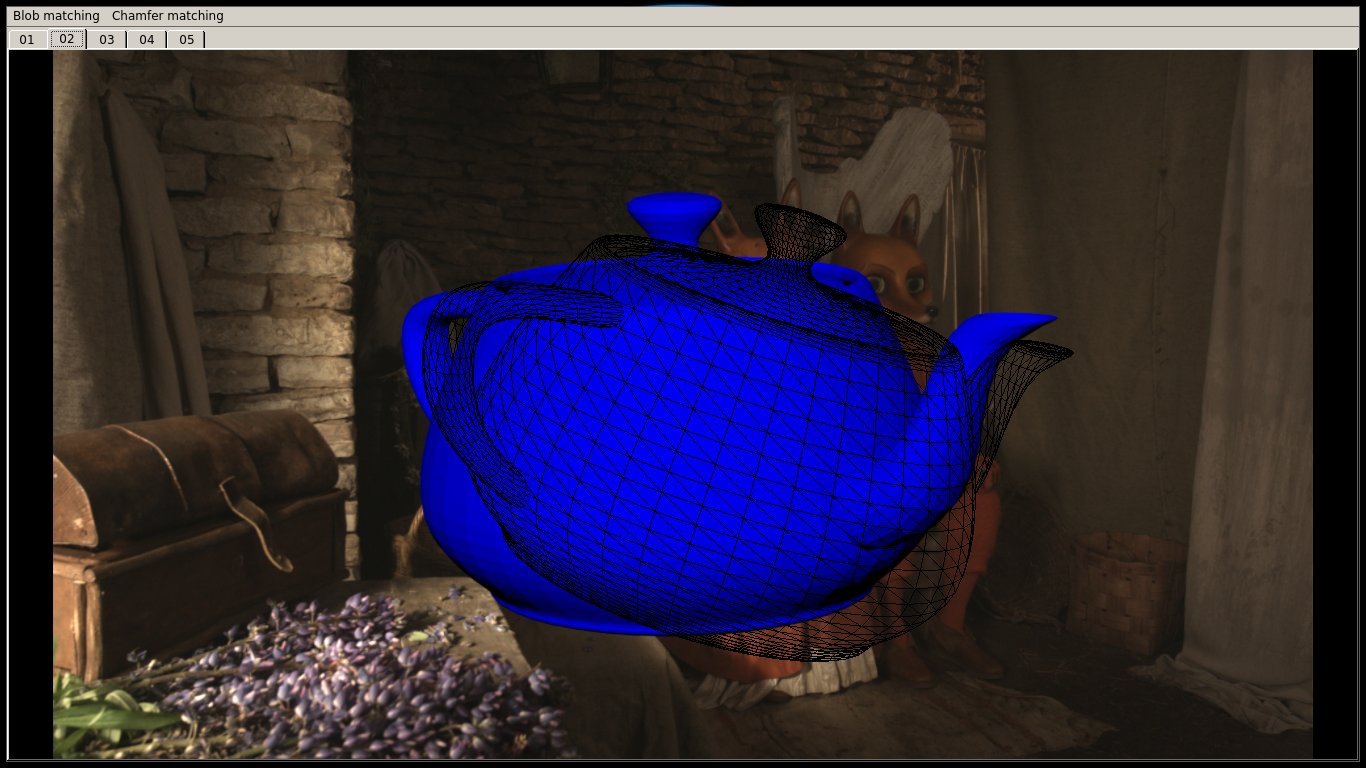
\includegraphics[height=6cm]{gui_samples/sample_02.png}
\end{frame}

\begin{frame}\frametitle{Склейка кода}
    Структура проекта
    \begin{itemize}
        \item main
        \item loading
        \item matching
            \begin{itemize}
                \item chamfer
                \item blob
            \end{itemize}
        \item gui
            \begin{itemize}
                \item main window
                \item key frame previewer
            \end{itemize}
    \end{itemize}
\end{frame}

\begin{frame}\frametitle{Результаты}
    \begin{itemize}
        \item Получился относительно цельный проект
        \item Все работает и шуршит
        \item Я разобрался с OpenGL и его использованием в Qt
        \item Получил опыт разработки в команде и работы с Github
    \end{itemize}
\end{frame}

\begin{frame}\frametitle{Chamfer matching}
    \begin{itemize}
        \item Задача: научиться по контуру предмета находить этот предмет на изображении.
        \pause
        \item Рассмотренный подход к решению описан в статье
        Ming-Yu Liu, Oncel Tuzel, Ashok Veeraraghavan, Rama Chellappa. Fast Directional Chamfer Matching
    \end{itemize}
\end{frame}

\begin{frame}\frametitle{Chamfer matching}
    \begin{center}
        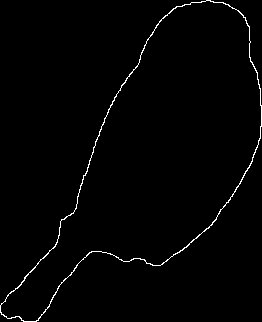
\includegraphics[height=4cm]{veselov_imgs/pattern3.jpg}
    \end{center}
\end{frame}

\begin{frame}\frametitle{Chamfer matching}
    \begin{center}
        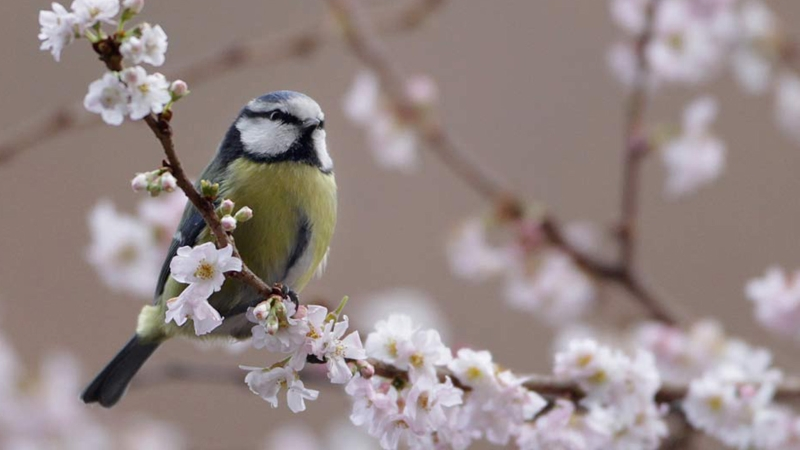
\includegraphics[height=6cm]{veselov_imgs/image3.jpg}
    \end{center}
\end{frame}

\begin{frame}\frametitle{Chamfer matching}
    \begin{center}
        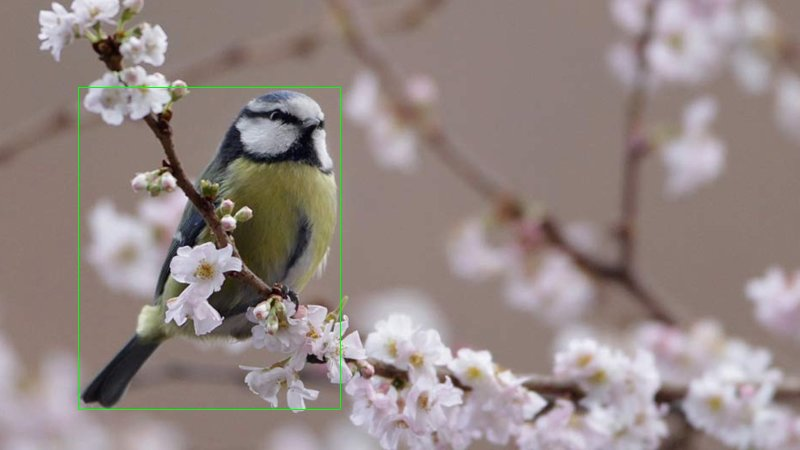
\includegraphics[height=6cm]{veselov_imgs/occurrence3.jpg}
    \end{center}
\end{frame}

\begin{frame}\frametitle{Алгоритм}
    \begin{itemize}
        \item С помощью алгоритма Кэнни найти на изображении границы между объектами.
        \pause
        \item Представить границы на изображении и контур предмета в виде набора отрезков.
        Такое представление удобно для дальнейших оптимизаций.
        \pause
        \item Для каждого возможного наложения контура на изображение посчитать эвристическую функцию отклонения.
        \pause
        \item Среди всех наложений выбрать одно с минимальным значением функции.
    \end{itemize}
\end{frame}

\begin{frame}\frametitle{Алгоритм Кэнни}
    \begin{itemize}
        \item Алгоритм Кэнни получает на вход изображение, как функцию интенсивности от двух переменных.
        \pause
        \item Для каждого пикселя вычисляется приближенное значение градиента этой функции в данном пикселе.
        \pause
        \item Пиксели с высоким значением модуля градиента объявляются граничными.
        \pause
        \item В работе был использован готовый алгоритм из библиотеки OpenCV.
    \end{itemize}
\end{frame}

\begin{frame}\frametitle{Алгоритм Кэнни, пример работы}
    \begin{center}
        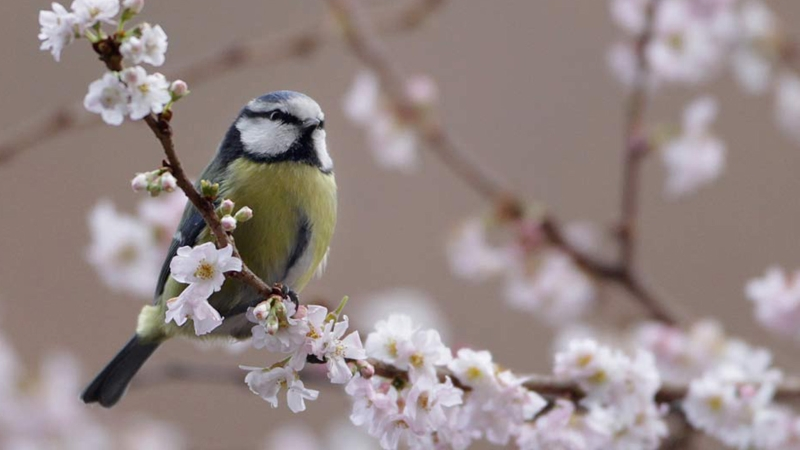
\includegraphics[height=6cm]{veselov_imgs/image3.jpg}
    \end{center}
\end{frame}

\begin{frame}\frametitle{Алгоритм Кэнни, пример работы}
    \begin{center}
        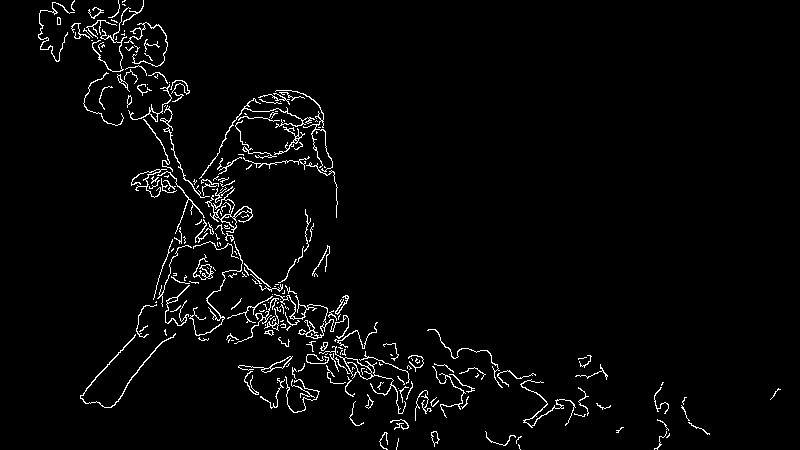
\includegraphics[height=6cm]{veselov_imgs/edge_map3.jpg}
    \end{center}
\end{frame}

\begin{frame}\frametitle{Линеаризация границ}
    \begin{itemize}
        \item Алгоритм Кэнни находит набор пикселей, которые являются граничными.
        \pause
        \item Необходимо приблизить этот набор пикселей отрезками. Дополнительно необходимо, чтобы
        все отрезки имели с осью координат один из $q$ равномерно расположенных на $[0, \pi)$ углов.
        Число $q$ должно быть небольшое.
        \pause
        \item Авторы статьи предлагают воспользоваться вариацией алгоритма RANSAC (Random sample consensus).
    \end{itemize}
\end{frame}

\begin{frame}\frametitle{RANSAC}
    \begin{itemize}
        \item Алгоритм Кэнни для каждого пикселя находит градиент интенсивности в этом пикселе.
        Если пиксель граничный, то градиент является нормалью к кривой границы.
        \pause
        \item Таким образом каждый пиксель $p$ задает прямую $l$, проходящую через него перпендикулярно нормали.
        Так как необходимо найти отрезок с одним из заданных углов, то считается, что $p$ задает прямую, угол которой
        наименее всего отличается от угла $l$.
        \pause
        \item Среди соседей $p$ отбираются пиксели, которые не слишком сильно
        удалены от прямой $l$. Этот процесс продолжается по цепочке.
        \pause
        \item Говоря иначе, из пикселя $p$ запускается обход в ширину.
        \pause
        \item Посещенные пиксели объявляются поддержкой гипотезы пикселя $p$.
        \pause
        \item На очередном шаге алгоритма случайным образом выбирается небольшое
        количество пикселей, для каждого из которых вычисляется поддержка.
        \pause
        \item Пиксель с наибольшей поддержкой и всеми пикселями, которые его поддержали, заменяются на отрезок.
    \end{itemize}
\end{frame}

\begin{frame}\frametitle{RANSAC, пример работы}
    \begin{center}
        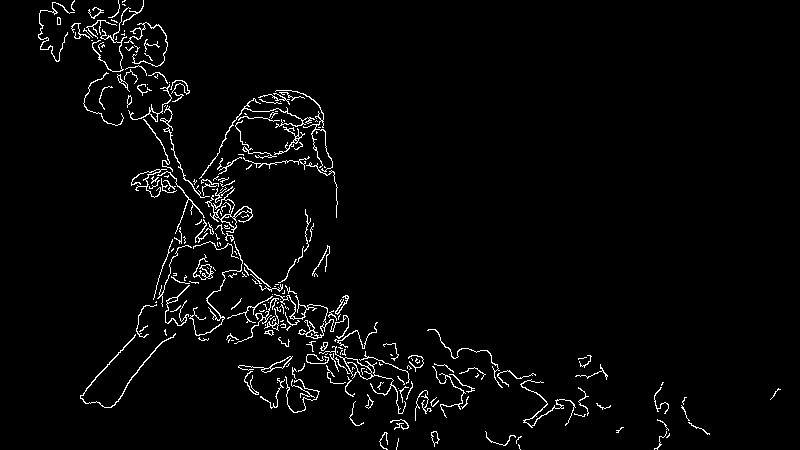
\includegraphics[height=6cm]{veselov_imgs/edge_map3.jpg}
    \end{center}
\end{frame}

\begin{frame}\frametitle{RANSAC, пример работы}
    \begin{center}
        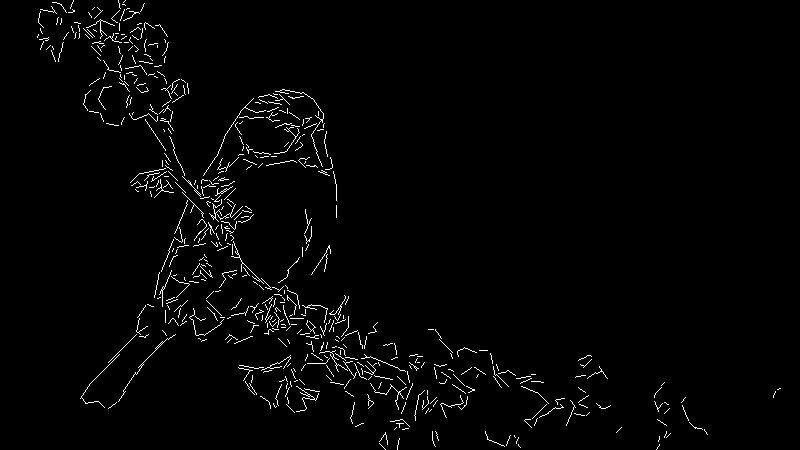
\includegraphics[height=6cm]{veselov_imgs/l_edge_map3.jpg}
    \end{center}
\end{frame}

\begin{frame}\frametitle{Линеаризация контура}
    \begin{itemize}
        \item К контуру предмета можно применить аналогичную идею.
        \pause
        \item Однако контур не является функцией интенсивности, и на нем нельзя запустить алгоритм Кэнни.
        \pause
        \item Как следствие, для каждого пикселя контура не известно направление по которому нужно откладывать прямую.
        \pause
        \item Поэтому нужно для каждого пикселя перебрать направление среди $q$ зафиксированных.
    \end{itemize}
\end{frame}

\begin{frame}\frametitle{Эвристическая функция}
    \begin{itemize}
        \item Пусть $p$ пиксель изображения, а $E$ -- множество граничных пикселей на изображении.
        Тогда обозначим $d(p) = \min\limits_{e \in E}\{dist(p, e)\}$, где $dist$ -- евклидов расстояни
        между точками.
        \pause
        \item Чем дальше пиксель из контура от граничных пикселей изображения при наложении, тем хуже наложение.
        \pause
        \item Поэтому за эвристическую функцию принимают $f = \sum\limits_{p}{d(p)}$, где $p$ пробегает
        все пиксели контура при его наложении на изображение.
    \end{itemize}
\end{frame}

\begin{frame}\frametitle{Оптимизации}
    \begin{itemize}
        \item Разумным подходом является заранее подсчитать для каждого пикселя
        $p$ величину $d(p) = \min\limits_{e \in E}\{dist(p, e)\}$.
        \pause
        \item Данную задача решается методом динамического программирования с
        применением идеи convex hull trick.
        \pause
        \item Для каждого из $q$ направлений можно посчитать массивы частичных сумм.
        Это позволит за $\mathcal{O}(1)$ времени суммировать $d(p)$ для всех
        $p$ из одного отрезка.
    \end{itemize}
\end{frame}

\begin{frame}\frametitle{Другой пример}
    \begin{center}
        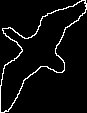
\includegraphics[height=3cm]{veselov_imgs/pattern1.jpg}\
        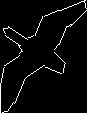
\includegraphics[height=3cm]{veselov_imgs/l_pttrn1.jpg}\\
        Изображения контуров увеличены.
    \end{center}
\end{frame}

\begin{frame}\frametitle{Другой пример}
    \begin{center}
        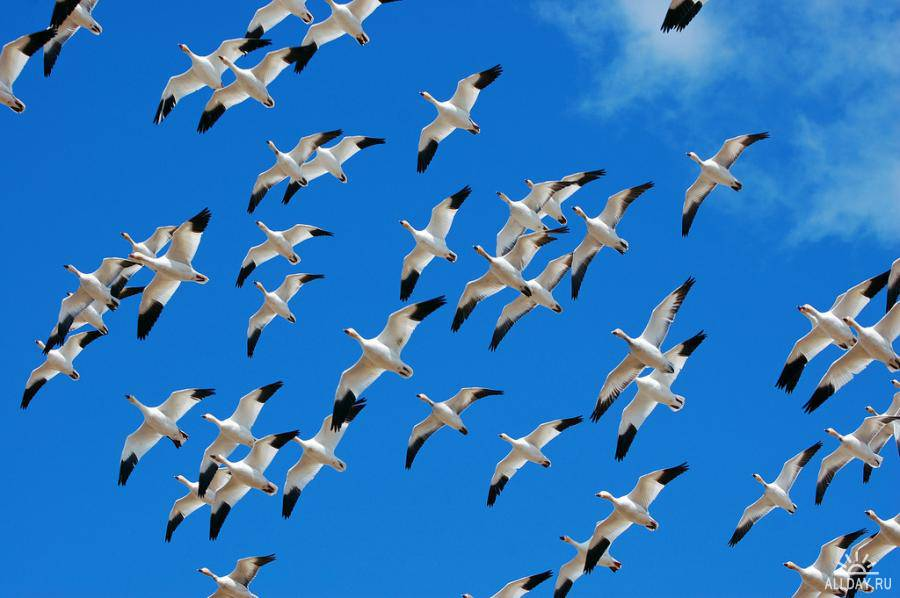
\includegraphics[height=6cm]{veselov_imgs/image1.jpg}
    \end{center}
\end{frame}

\begin{frame}\frametitle{Другой пример}
    \begin{center}
        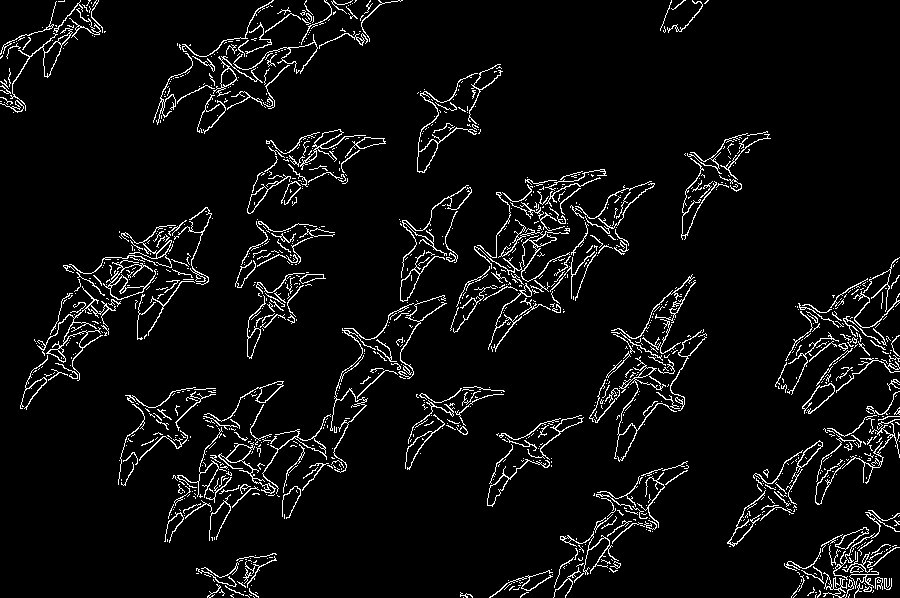
\includegraphics[height=6cm]{veselov_imgs/edge_map1.jpg}
    \end{center}
\end{frame}

\begin{frame}\frametitle{Другой пример}
    \begin{center}
        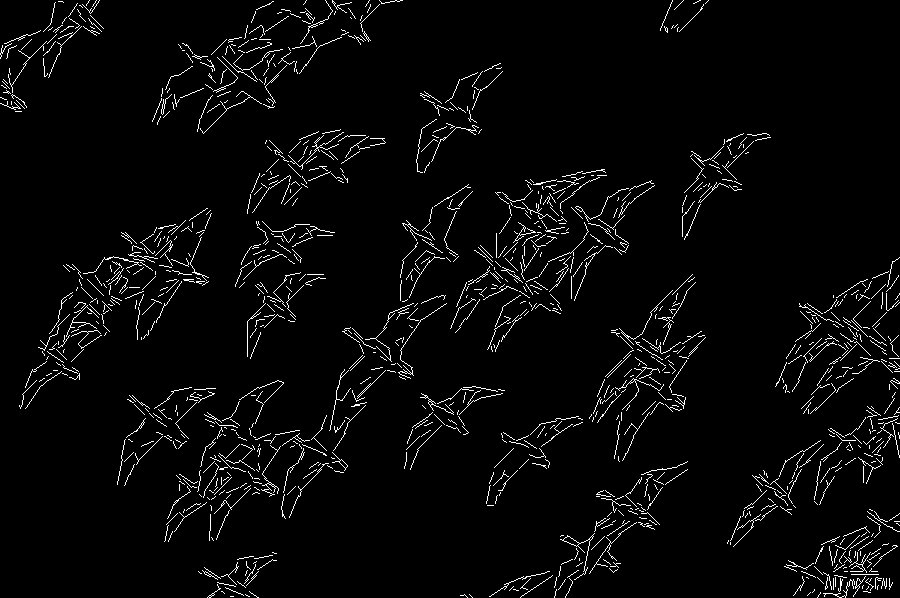
\includegraphics[height=6cm]{veselov_imgs/l_edge_map1.jpg}
    \end{center}
\end{frame}

\begin{frame}\frametitle{Другой пример}
    \begin{center}
        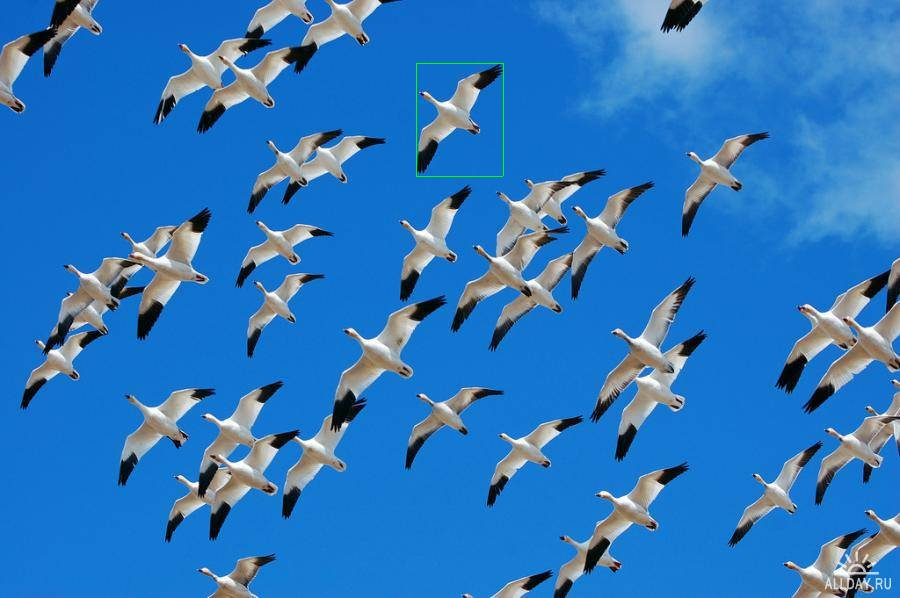
\includegraphics[height=6cm]{veselov_imgs/occurrence1.jpg}
    \end{center}
\end{frame}

\begin{frame}\frametitle{Что еще можно сделать?}
    \begin{itemize}
        \item Авторы статьи Fast Directional Chamfer Matching предлагают
        немного изменить классическую эвристическую функцию.\\
        Вместо $f = \sum\limits_{p}{d(p)}$, предлагается $f' = \sum\limits_{p}{\bigg[d(p) + \lambda angle(p)\bigg]}$,
        где $angle(p)$ разница между направлениями (углами) градиента в ближайшем к $p$ граничном пикселе
        и пикселе контура, который при наложении перешел в $p$, а $\lambda$ коэффициента влияния нового слагаемого.
        \pause
        \item Провести исследование на большом количестве тестов, чтобы понять, можно ли где-то что-то улучшить.
    \end{itemize}
\end{frame}

\begin{frame}\frametitle{Недостатки Chamfer matching}
    \begin{itemize}
        \item Необходимость в точном контуре.\\
        Если контур будет неправильно повернут или будет иметь
        неправильный размер, то Chamfer matching не сработает.
        \pause
        \item Неустойчивость к помехам.
    \end{itemize}
\end{frame}

\begin{frame}\frametitle{Неустойчивость к помехам}
    \begin{center}
        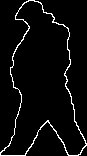
\includegraphics[height=3cm]{veselov_imgs/pattern2.jpg}\
        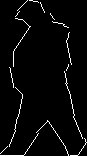
\includegraphics[height=3cm]{veselov_imgs/l_pttrn2.jpg}\\
        Изображения контуров увеличены.
    \end{center}
\end{frame}

\begin{frame}\frametitle{Неустойчивость к помехам}
    \begin{center}
        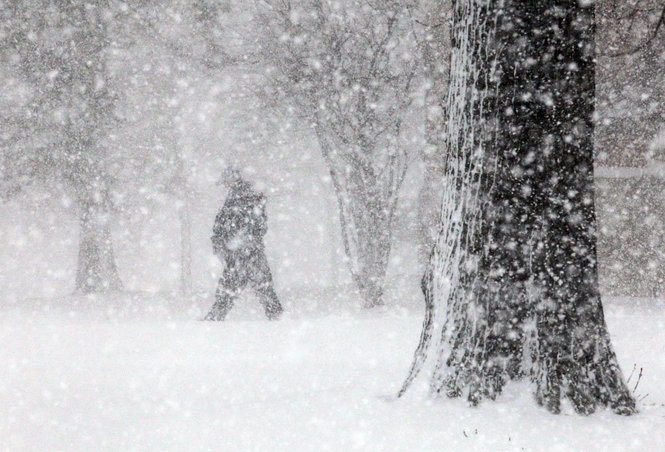
\includegraphics[height=6cm]{veselov_imgs/image2.jpg}
    \end{center}
\end{frame}

\begin{frame}\frametitle{Неустойчивость к помехам}
    \begin{center}
        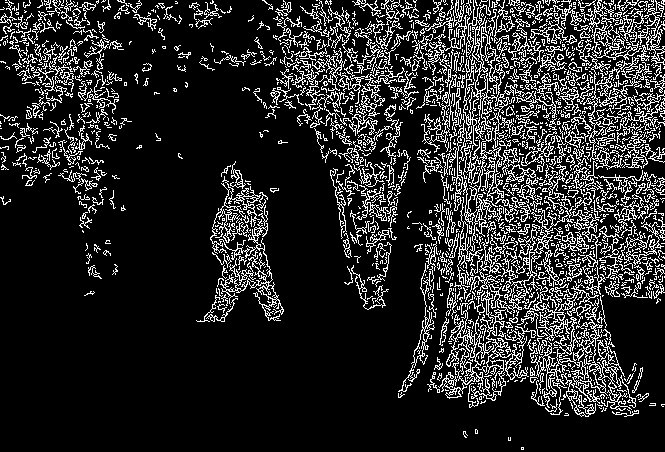
\includegraphics[height=6cm]{veselov_imgs/edge_map2.jpg}
    \end{center}
\end{frame}

\begin{frame}\frametitle{Неустойчивость к помехам}
    \begin{center}
        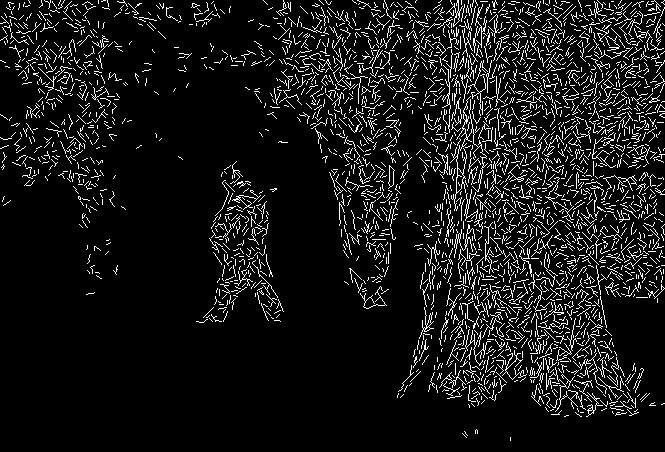
\includegraphics[height=6cm]{veselov_imgs/l_edge_map2.jpg}
    \end{center}
\end{frame}

\begin{frame}\frametitle{Неустойчивость к помехам}
    \begin{center}
        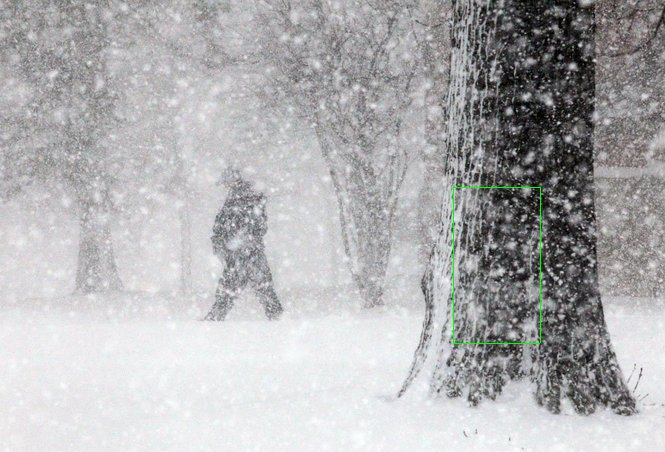
\includegraphics[height=6cm]{veselov_imgs/occurrence2.jpg}
    \end{center}
\end{frame}

\begin{frame}\frametitle{Заключение о Chamfer matching}
    Во время работы над проектом:
    \begin{itemize}
        \item Были изучены статьи на тему
        <<компьютерного зрения>> (Chamfer matching, Canny algorithm), а также
        вероятностного поиска некоторой модели среди помех (RANSAC).
        
        \item Была написана реализация Chamfer matching на языке Python с
        использованием пакетов numpy и cv2.
        
        \item Для хранения исходного кода использовался GitHub.
    \end{itemize}
\end{frame}

\begin{frame}\frametitle{Chamfer matching}
    \begin{itemize}
        \item Задача: научиться по контуру предмета находить этот предмет на изображении.
        \pause
        \item Рассмотренный подход к решению описан в статье
        Ming-Yu Liu, Oncel Tuzel, Ashok Veeraraghavan, Rama Chellappa. Fast Directional Chamfer Matching
    \end{itemize}
\end{frame}

\begin{frame}\frametitle{Алгоритм}
    \begin{itemize}
        \item С помощью алгоритма Кэнни найти на изображении границы между объектами.
        \pause
        \item Представить границы на изображении и контур предмета в виде набора отрезков.
        Такое представление удобно для дальнейших оптимизаций.
        \pause
        \item Для каждого возможного наложения контура на изображение посчитать эвристическую функцию отклонения.
        \pause
        \item Среди всех наложений выбрать одно с минимальным значением функции.
    \end{itemize}
\end{frame}

\begin{frame}\frametitle{Алгоритм Кэнни}
    \begin{itemize}
        \item Алгоритм Кэнни получает на вход изображение, как функцию интенсивности от двух переменных.
        \pause
        \item Для каждого пикселя вычисляется приближенное значение градиента этой функции в данном пикселе.
        \pause
        \item Пиксели с высоким значением модуля градиента объявляются граничными.
        \pause
        \item В работе был использован готовый алгоритм из библиотеки OpenCV.
    \end{itemize}
\end{frame}


\begin{frame}\frametitle{Неустойчивость к помехам}
    \begin{center}
        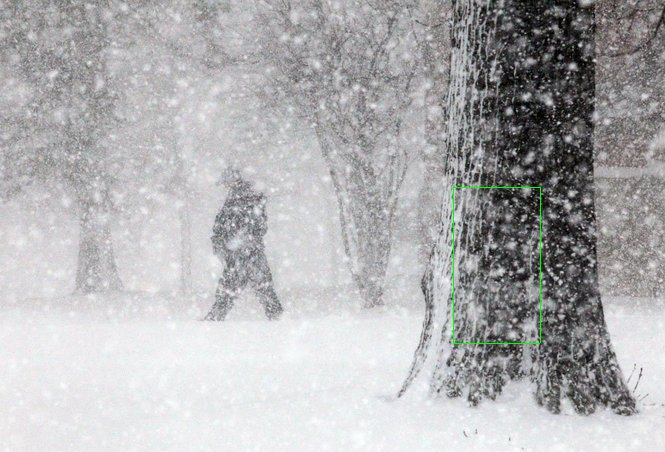
\includegraphics[height=6cm]{veselov_imgs/occurrence2.jpg}
    \end{center}
\end{frame}

\begin{frame}\frametitle{Заключение о Chamfer matching}
    Во время работы над проектом:
    \begin{itemize}
        \item Были изучены статьи на тему
        <<компьютерного зрения>> (Chamfer matching, Canny algorithm), а также
        вероятностного поиска некоторой модели среди помех (RANSAC).
        
        \item Была написана реализация Chamfer matching на языке Python с
        использованием пакетов numpy и cv2.
        
        \item Для хранения исходного кода использовался GitHub.
    \end{itemize}
\end{frame}

Задача
Алгоритм
-Определение ключевых точек
-Сопоставление ключевых точек
-PnP
-склонен к ошибкам, поэтому RANSAC (Random sample consensus)
Определение ключевых точек
-Точки, которые обладают некоторыми важными свойствами
-Устойчивость к деформациям, точность локализации
Сопоставление ключевых точек
-Вычисление дескрипторов (вектор 128)
-Сопоставление точек расстояние между дескрипторами которых минимально
RANSAC



\begin{frame}
    \begin{center}
        Спасибо за внимание! \\
        \includegraphics[width=0.5\textwidth]{qr.eps} \\
        \url{https://github.com/ReptoidBusters/object-detection}
    \end{center}
\end{frame}

\end{document}
